\documentclass[a4paper, 12pt]{report}

\usepackage{charter}
\usepackage{makeidx}
\usepackage{fancyhdr}
\usepackage{hyperref}
\usepackage[utf8]{inputenc}
\usepackage{graphicx}
\usepackage[left=2cm, right=2cm]{geometry}
\usepackage{latexsym}
\usepackage{amsmath, amsthm, amssymb}
\usepackage{rotating}


\begin{titlepage}
\title{Disegno del sistema}
\author{Release 0.4}
\date{\today \\Firenze \\\begin{figure}[h] \centering 
\includegraphics[width=0.2\textwidth]{../images/logokiwi.png} \end{figure} }
\end{titlepage}

\pagestyle{fancy}

\begin{document}

\maketitle

\section*{Approvazione, redazione, lista distribuzione}
\begin{table}[h!]
  \begin{center}
    \begin{tabular}{| l | l | p{60mm} |}
    \hline
    \textbf{approvato da} & \textbf{il giorno} & \textbf{firma} \\
	\hline    
	Marco Tinacci & \today &  \\
    \hline
    \end{tabular}
  \end{center}
\end{table}

\begin{table}[h!]
  \begin{center}
    \begin{tabular}{| l | l | p{60mm} |}
    \hline
    \textbf{redatto da} & \textbf{il giorno} & \textbf{firma} \\
	\hline    
	Francesco Calabri & \today &  \\
    \hline
	Niccol\`o Rogai & \today &  \\
    \hline
	Marco Tinacci & \today &  \\
    \hline
    \end{tabular}
  \end{center}
\end{table}

\begin{table}[h!]
  \begin{center}
    \begin{tabular}{| l | l | p{60mm} |}
    \hline
    \textbf{distribuito a} & \textbf{il giorno} & \textbf{firma} \\
	\hline    
	Francesco Calabri & \today &  \\
    \hline
	Manuele Paulantonio & \today &  \\
    \hline
	Daniele Poggi & \today &  \\
    \hline
	Massimo Nocentini & \today &  \\
    \hline
	Niccol\`o Rogai & \today &  \\
    \hline
	Marco Tinacci & \today &  \\
    \hline
    \end{tabular}
  \end{center}
\end{table}

\tableofcontents

\newpage

\section{Introduzione}
In questo documento viene illustrata l'architettura del modulo tramite le viste dei \emph{class diagrams} e i \emph{sequence diagrams}, come evoluzione naturale, rispettivamente di \emph{domain model} e \emph{use cases} appartenenti al linguaggio \emph{UML 2.0}. \\
I diagrammi delle classi servono quindi a individuare le strutture dei dati e i metodi assiociati mentre quelli di sequenza evidenziano le comunicazioni che intercorrono tra le entit\`a. \\
Per semplificare la rappresentazione del diagramma delle classi abbiamo deciso di scrivere gli attributi privati con la notazione di quelli pubblici ``+ attribute'' dando per assunto che siano provvisti dei metodi pubblici di ``getAttribute()'' e ``setAttribute()''. \\

\chapter{Class Diagrams}
\section{Commons}
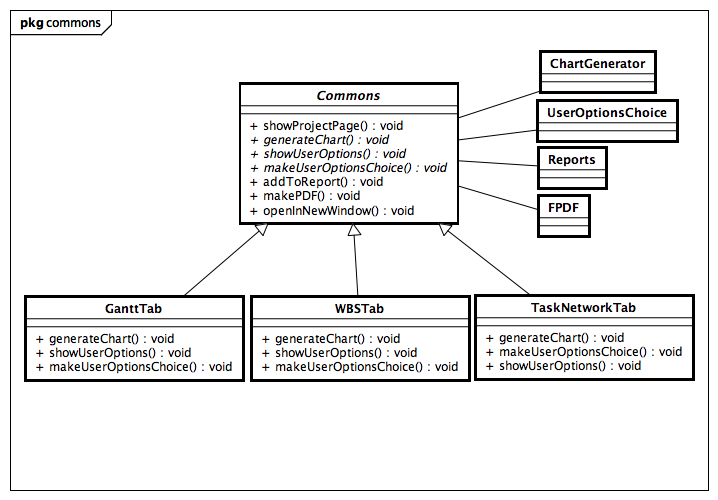
\includegraphics[width=\textwidth]{diagramma_classe/commons.png}
La classe common racchiude tutte le funzioni principali del modulo. Utilizza le classi
\begin{itemize}
	\item ChartGenerator
	\item UserOptionsChoice
	\item Reports
	\item FPDF (esterna al modulo e gi\`a utilizzata in PMango)
\end{itemize}
A seconda di quale tab viene caricato, pu\`o essere usata l'estensione di Commons corrispondente: 
\begin{itemize}
	\item GanttTab
	\item WBSTab
	\item TaskNetworkTab
\end{itemize}
che implementano la generazione del diagramma, la creazione della maschera delle user options e l'acquisizione delle scelte dei parametri.
\section{Chart Generator}
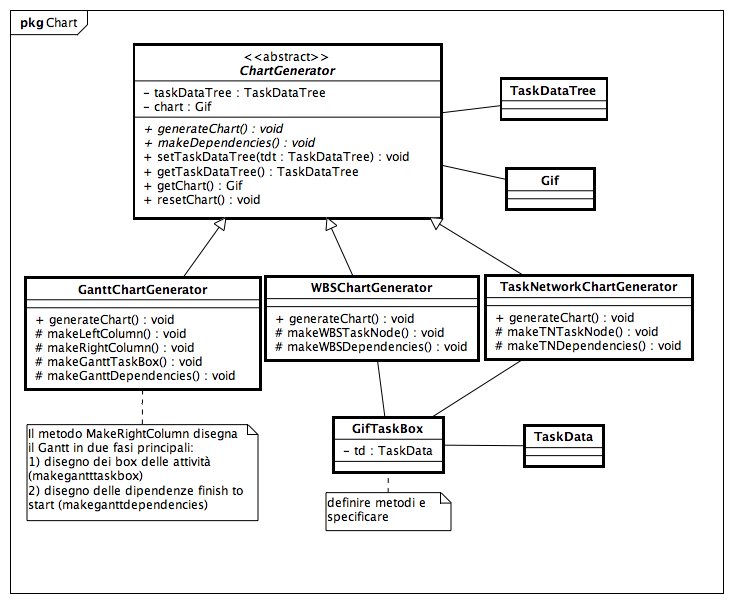
\includegraphics[width=\textwidth]{diagramma_classe/chart.png}
\section{Task Data}
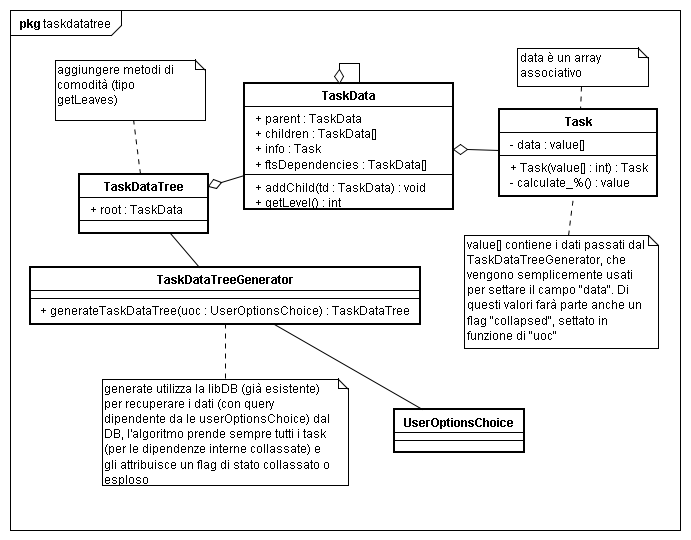
\includegraphics[width=\textwidth]{diagramma_classe/taskdatatree.png}
\section{User Options}
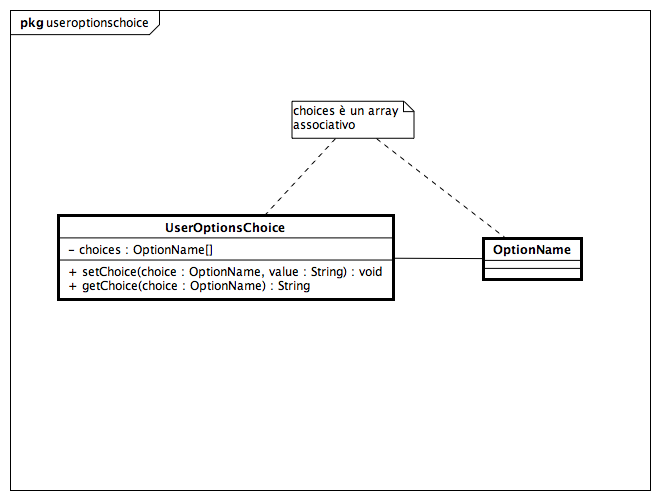
\includegraphics[width=\textwidth]{diagramma_classe/useroptionschoice.png}
\begin{itemize}
	\item UserOptionsChoice: la classe che racchiude le scelte fatte dall'utente in un array associativo controllato dai metodi get e set.
	\item OptionName: un'enumerate che vincola l'accesso all'array associativo ai soli campi specificati. Questa contiene le seguenti voci (associate ai possibili valori che possono assumere):
	\begin{itemize}
		\item TaskNameOption: boolean		
		\item PlannedTimeFrameOption: boolean
		\item ActualTimeFrameOption: boolean
		\item PlannedDataOption: boolean
		\item ActualDataOption: boolean
		\item CompletitionBarOption: boolean
		\item AlertMarkUserOption: boolean
		\item WBSExplosionLevelUserOption: numeric
		% da completare
		\item WBSUserSpecificationUserLevel: ??
		\item ReplicateArrowUserOption: ??
		\item FindCriticalPathUserOption: boolean
		\item CriticalPathTableUserOption: boolean
		\item ResourcesDetailsOption: boolean
		\item CompleteDiagramUserOptions: ??
		\item WBSTreeSpecification: LevelSpecification, UserCustomSpecification
		\item TimeGrain: HourlyGrain, DailyGrain, WeaklyGrain, MonthlyGrain, YearlyGrain
		\item ImageDimensionUserOption: CustomDim, FitInWindowDim, OptionalDim, DefaultDim 
		\item TimeRangeUserOption: CustomRange, WholeProjectRange, FromStartRange, ToEndRange
	\end{itemize}
	Il significato di questi parametri sono specificati nei casi d'uso.
	% se inseriti valori errati ricondurre a quelli di default
\end{itemize}
\section{Reports}
% diagramma
\chapter{Sequence Diagrams}

\end{document}
